% Section owner: Akhil (DL dataset pipeline and augmentation)
\section{Dataset and Augmentation}
\label{sec:p2data}
We use the Phase 1 split without change: 54{,}000 training and 6{,}000 validation images drawn from the official
training set with stratification and seed 42, and the 10{,}000 official test images. The pipeline recomputes the
split and compares its SHA-256 hash with the hash stored in Phase 1. Pixels are scaled to $[0,1]$ and standardised
with the mean and standard deviation of the training split only.

Augmentation is applied to training batches only, on the training device and on whole batches at once
(Fig.~\ref{fig:p2aug}). Each operation preserves the label and produces an image that could plausibly occur.
\begin{itemize}
\item \emph{Random crop}: the image is padded by 2 pixels with the background value and a random $28\times28$ window
is cut, a shift of up to $\pm2$ pixels. Padding uses the standardised value of a black pixel so that no gray frame
appears.
\item \emph{Horizontal flip} with probability 0.5. Garments are close to symmetric, and all footwear in the dataset
points the same way, so the benefit of the flip is an empirical question.
\item \emph{Random erasing}~\cite{zhong2020random}: with probability 0.25 a random rectangle covering 2--20\% of the
image is overwritten with the dataset mean.
\end{itemize}
Vertical flips and rotations are excluded because the catalogue images are upright. Validation and test images are
never augmented.

\begin{figure}[t]
\centering
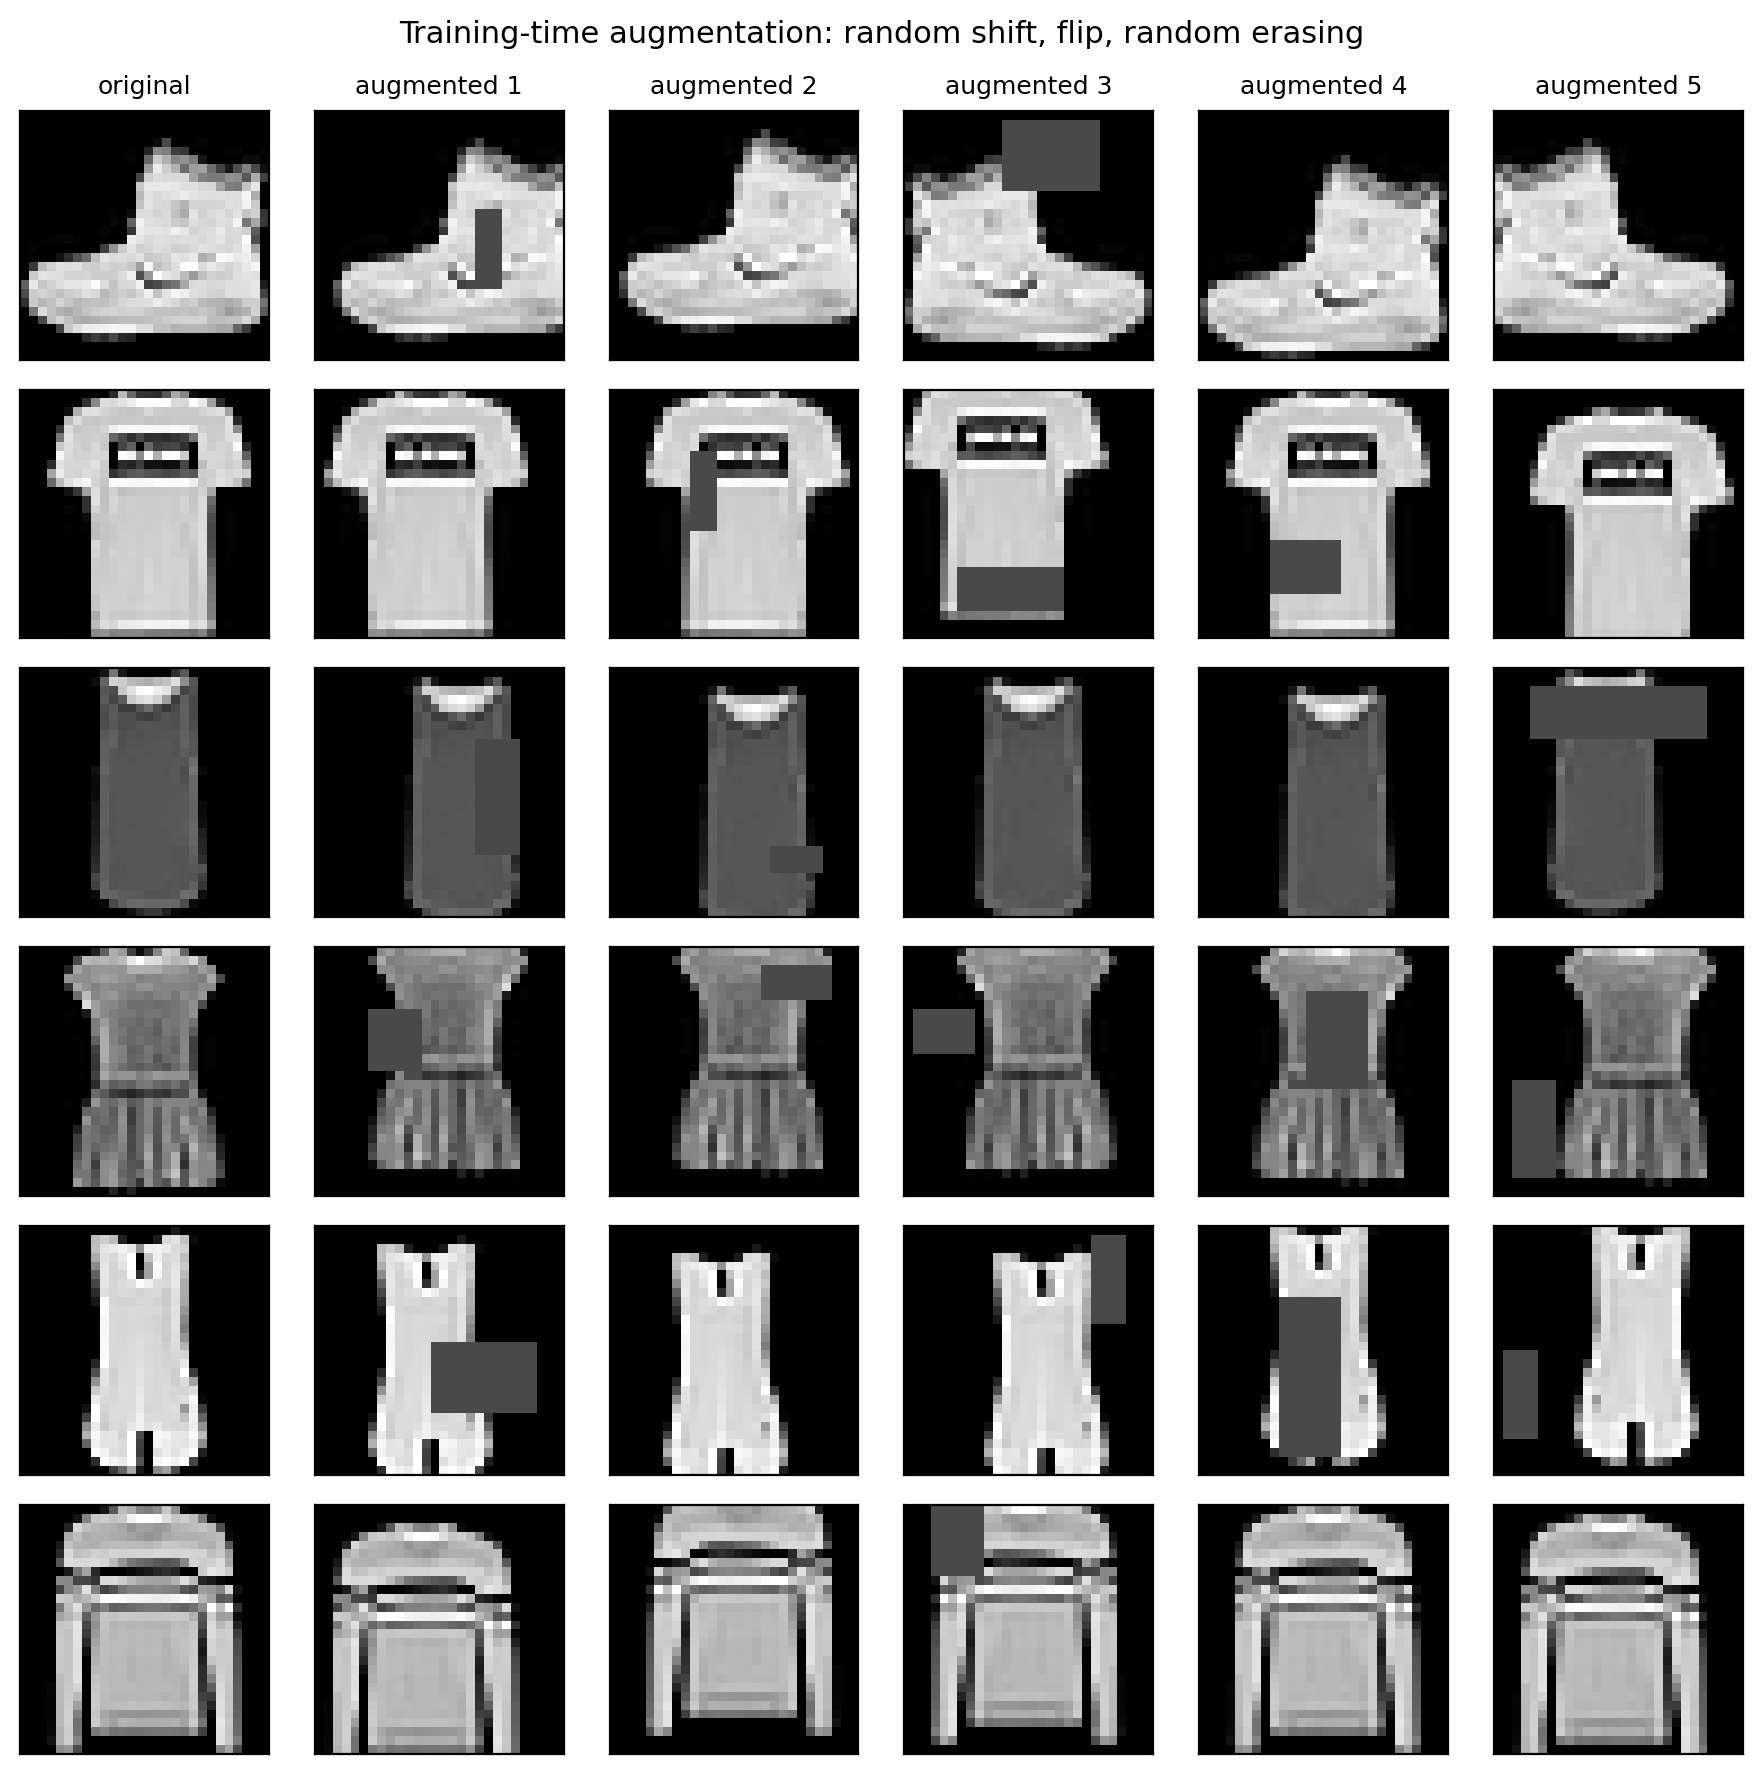
\includegraphics[width=\columnwidth]{augmentation_examples.png}
\caption{Training images (left column) and five augmented versions of each. Erasing is shown with a higher
probability than in training so that every row contains an example.}
\label{fig:p2aug}
\end{figure}
